\documentclass{article}

\usepackage{graphicx}
\usepackage{tikz}
\usepackage{tikzsymbols}
\usetikzlibrary{calc,patterns,shapes.geometric}
\pagestyle{empty}
\usepackage[margin=0pt]{geometry}
\geometry{papersize={14in,12in}}

\def\centerarc[#1](#2)(#3:#4:#5){\draw[#1] ($(#2)+({#5*cos(#3)},{#5*sin(#3)})$) arc (#3:#4:#5);}

\begin{document}
	\begin{figure}
		\centering
		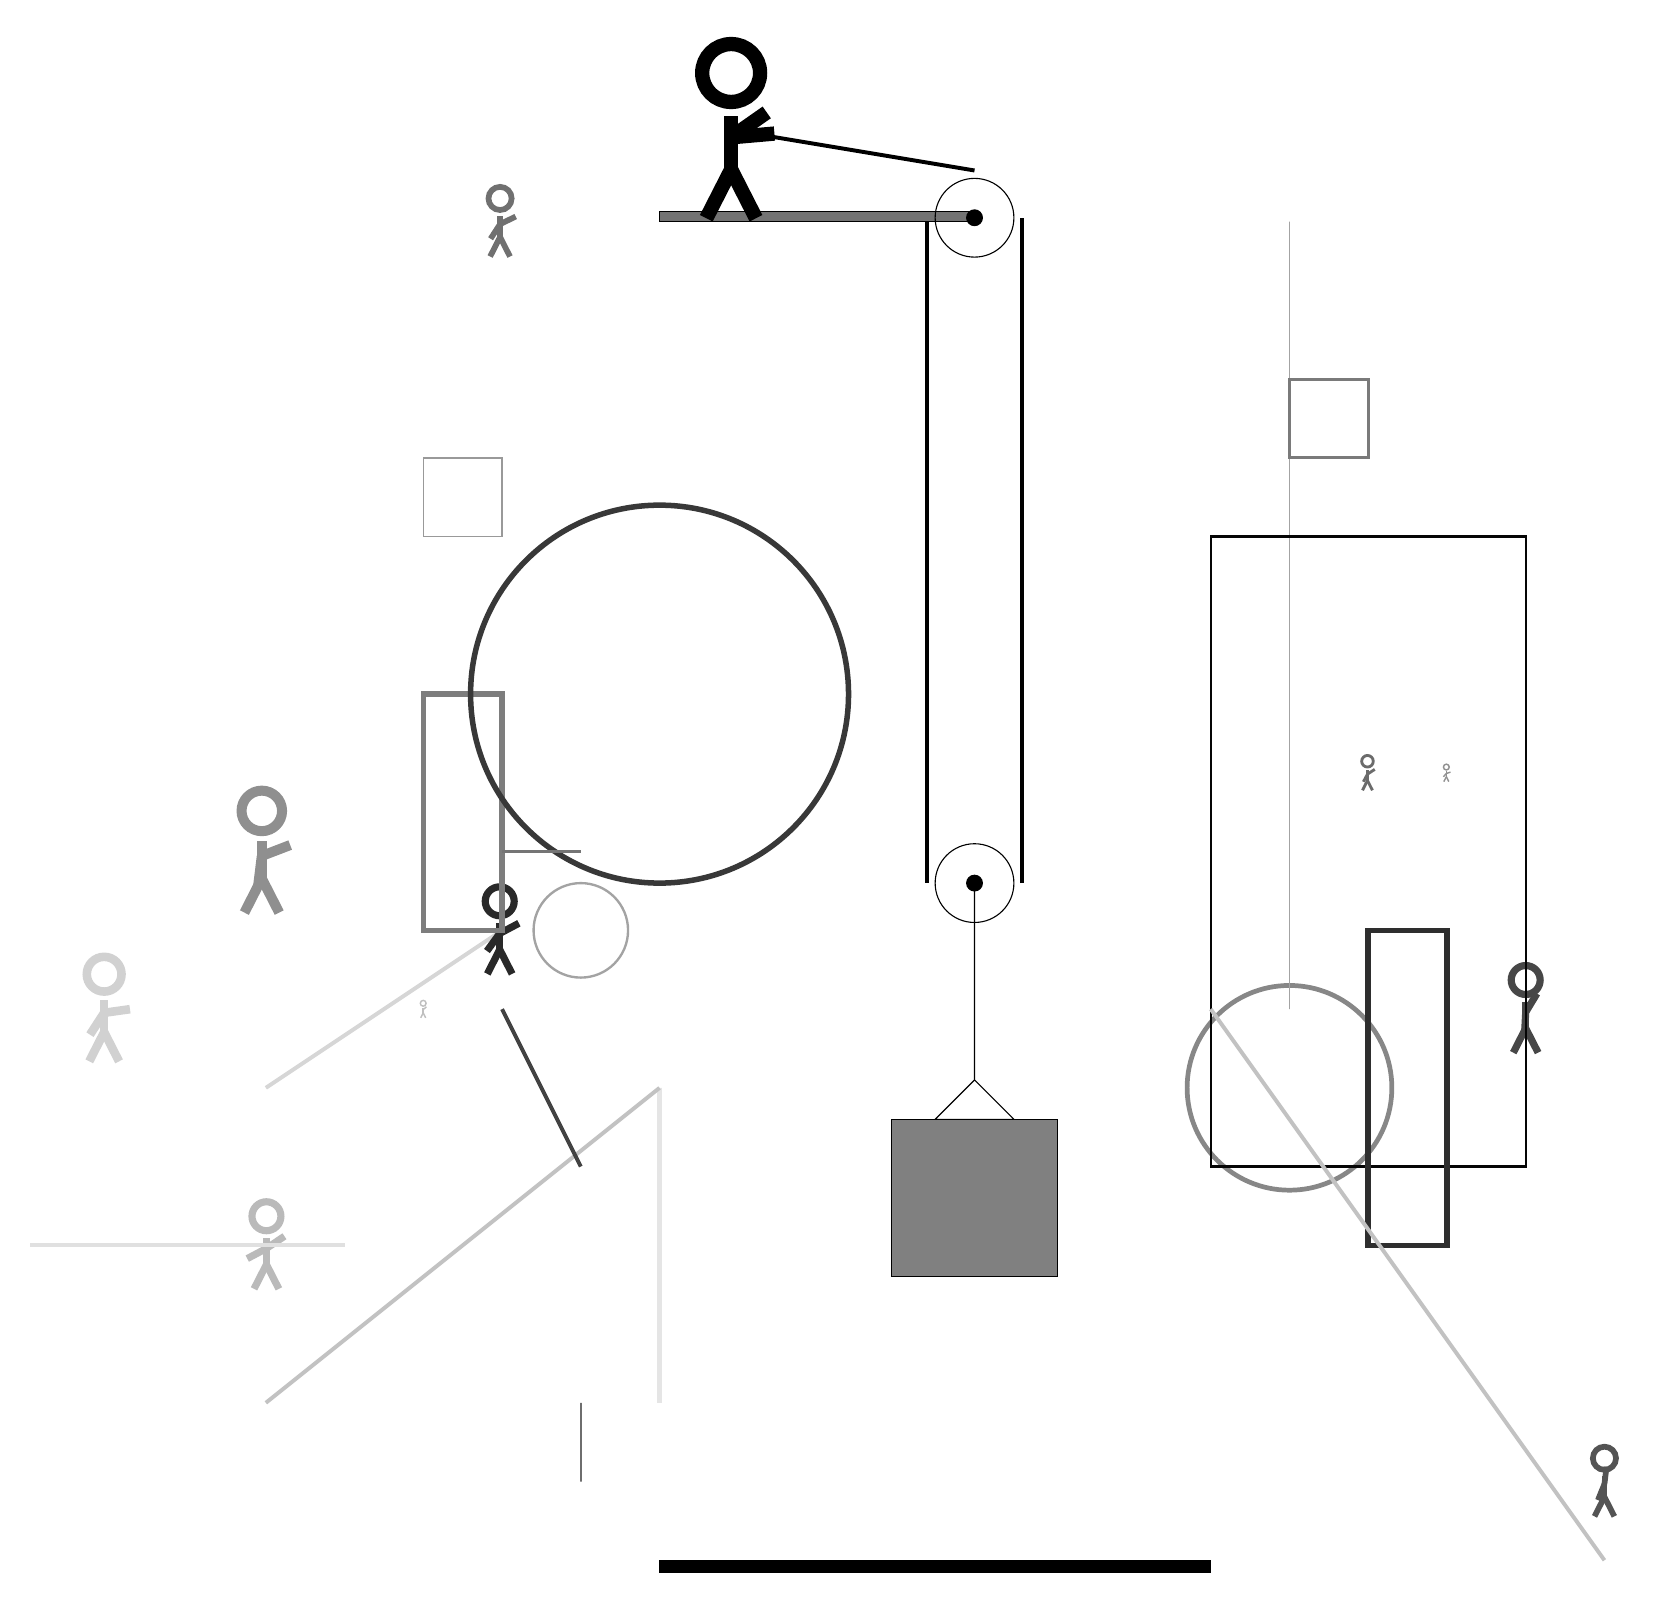
\begin{tikzpicture}
			%%%%% START %%%%%
			
			\draw[fill=black!55] (-2, 14) rectangle (2, 14.125);
			
			\draw (2, 5.6) circle (0.5);
			\draw[fill=black] (2, 5.6) circle (0.1);
			
			\draw (2, 14.05) circle (0.5);
			\draw[fill=black] (2, 14.05) circle (0.1);
			
			\draw (2, 5.6) -- (2, 3.1) -- (1.5, 2.6) -- (2.5, 2.6) -- (2, 3.1);
			\draw[fill=black!50] (0.95, 2.6) rectangle (3.05, 0.6);
			
			\draw[line width=0.5mm] (1.4, 14) -- (1.4, 5.6);
			\centerarc[line width=0.5mm](2, 5.6)(180:360:0.6);
			\draw[line width=0.5mm](2.6, 5.6) -- (2.6, 14.05);
			\centerarc[line width=0.5mm](2, 14.05)(0:90:0.6);
			\draw[line width=0.5mm](2, 14.65) -- (-1, 15.15);
			
			\draw[line width=0.5mm, color=black!16](-4, 5) -- (-7, 3);
			
			\draw [line width=0.6mm, color=black!47](6, 3) circle (1.3);
			\node[line width=0.3mm, color=black!25] at (-5, 4) {\Strichmaxerl[1][90][43]};
			\draw[line width=0.2mm, color=black!36] (6, 4) rectangle (6, 14);
			\node[line width=0.7mm, color=black!58] at (7, 7) {\Strichmaxerl[2][62][33]};
			\draw[line width=0.5mm, color=black!90](-6, 9) -- (-6, 9);
			\node[line width=0.3mm, color=black!43] at (8, 7) {\Strichmaxerl[1][48][18]};
			
			\node[line width=0.5mm, color=black!56] at (-4, 14) {\Strichmaxerl[4][57][26]};
			\draw[line width=0.7mm, color=black!10] (-2, -1) rectangle (-2, 3);
			\node[line width=0.3mm, color=black!84] at (-4, 5) {\Strichmaxerl[5][54][28]};
			\draw[line width=0.7mm, color=black!51] (-4, 5) rectangle (-5, 8);
			\draw[line width=0.3mm, color=black!57] (-3, -2) rectangle (-3, -1);
			\draw[line width=0.5mm, color=black!24](-2, 3) -- (-7, -1);
			
			\node[line width=0.4mm, color=black!72] at (9, 4) {\Strichmaxerl[5][87][59]};
			\draw[line width=0.5mm, color=black!74](-3, 2) -- (-4, 4);
			\draw[line width=0.3mm, color=black!98] (5, 10) rectangle (9, 2);
			\node[line width=0.4mm, color=black!18] at (-9, 4) {\Strichmaxerl[6][57][8]};
			\draw[line width=0.2mm, color=black!40] (-4, 10) rectangle (-5, 11);
			\draw [line width=0.7mm, color=black!78](-2, 8) circle (2.4);
			
			\node[line width=0.4mm, color=black!27] at (-7, 1) {\Strichmaxerl[5][28][34]};
			\draw [line width=0.3mm, color=black!36](-3, 5) circle (0.6);
			
			\node[line width=0.2mm, color=black!44] at (-7, 6) {\Strichmaxerl[7][83][21]};
			\draw[line width=0.4mm, color=black!54] (-3, 6) rectangle (-4, 6);
			\draw[line width=0.5mm, color=black!12](-6, 1) -- (-10, 1);
			\node[line width=0.6mm, color=black!67] at (10, -2) {\Strichmaxerl[4][68][83]};
			
			\draw[line width=0.7mm, color=black!82] (7, 5) rectangle (8, 1);
			
			\draw[line width=0.4mm, color=black!52] (6, 12) rectangle (7, 11);
			\draw[line width=0.5mm, color=black!24](10, -3) -- (5, 4);
			
			\node at (-1, 15.15) {\Strichmaxerl[10][-175][35]};
			
			\draw[fill=black] (-2, -3) rectangle (5, -3.15);
			
			%%%%% END %%%%%
		\end{tikzpicture}
	\end{figure}	
\end{document}